\subsubsection{Shopping List Browser}
The Shopping List Browser was implemented as follows:
\begin{description}
\item[Shopping List Creator] This was implemented with ShoppingList, a
PopupPanel which allows the user to add products to their shopping list via a
SuggestBox~\cite{suggest}. This then sends the request for stores which stock
the products to the Datastore via WebPage, WebSystem and RPC and directs the
user to Store Viewer once it has received a response.
\item[Store Viewer] This was implemented as BranchList which presents the user
with a tabular display of the stores which stock the products on their shopping
list along with the total cost of the shopping list. It contains buttons to access
 ShoppingListDetail and the Directions Viewer.
\item[Shopping List Viewer] This was implemented as ShoppingListDetail, a table
which displays the shopping list for a particular Branch. It therefore allows
the user to see the price and other details of each product.
It contains a button to access the Graph Viewer.
\end{description}
\begin{figure}[h!]
\centering
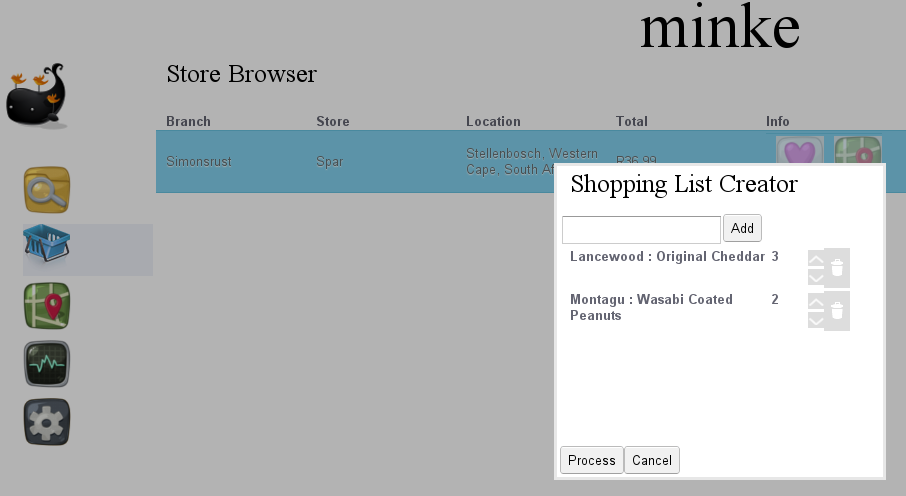
\includegraphics[width=0.8\textwidth]{gwt-list.png}
\caption{The Shopping List Creator with the Store Viewer in the background.}
\end{figure}